% Generated by render-figures.mjs from scene.mjs and figures.mjs.
\documentclass[tikz,border=0pt]{standalone}
\usepackage{xcolor}
\definecolor{bg}{HTML}{1B1F27}
\definecolor{fg}{HTML}{E6EDF3}
\definecolor{dim}{HTML}{9AA5B1}
\definecolor{c1}{HTML}{7BC47F}
\definecolor{c2}{HTML}{E5826F}
\definecolor{prediction}{HTML}{6EA8FE}
\definecolor{observed}{HTML}{F0C060}
\definecolor{epipolar}{HTML}{B39DDB}
\begin{document}
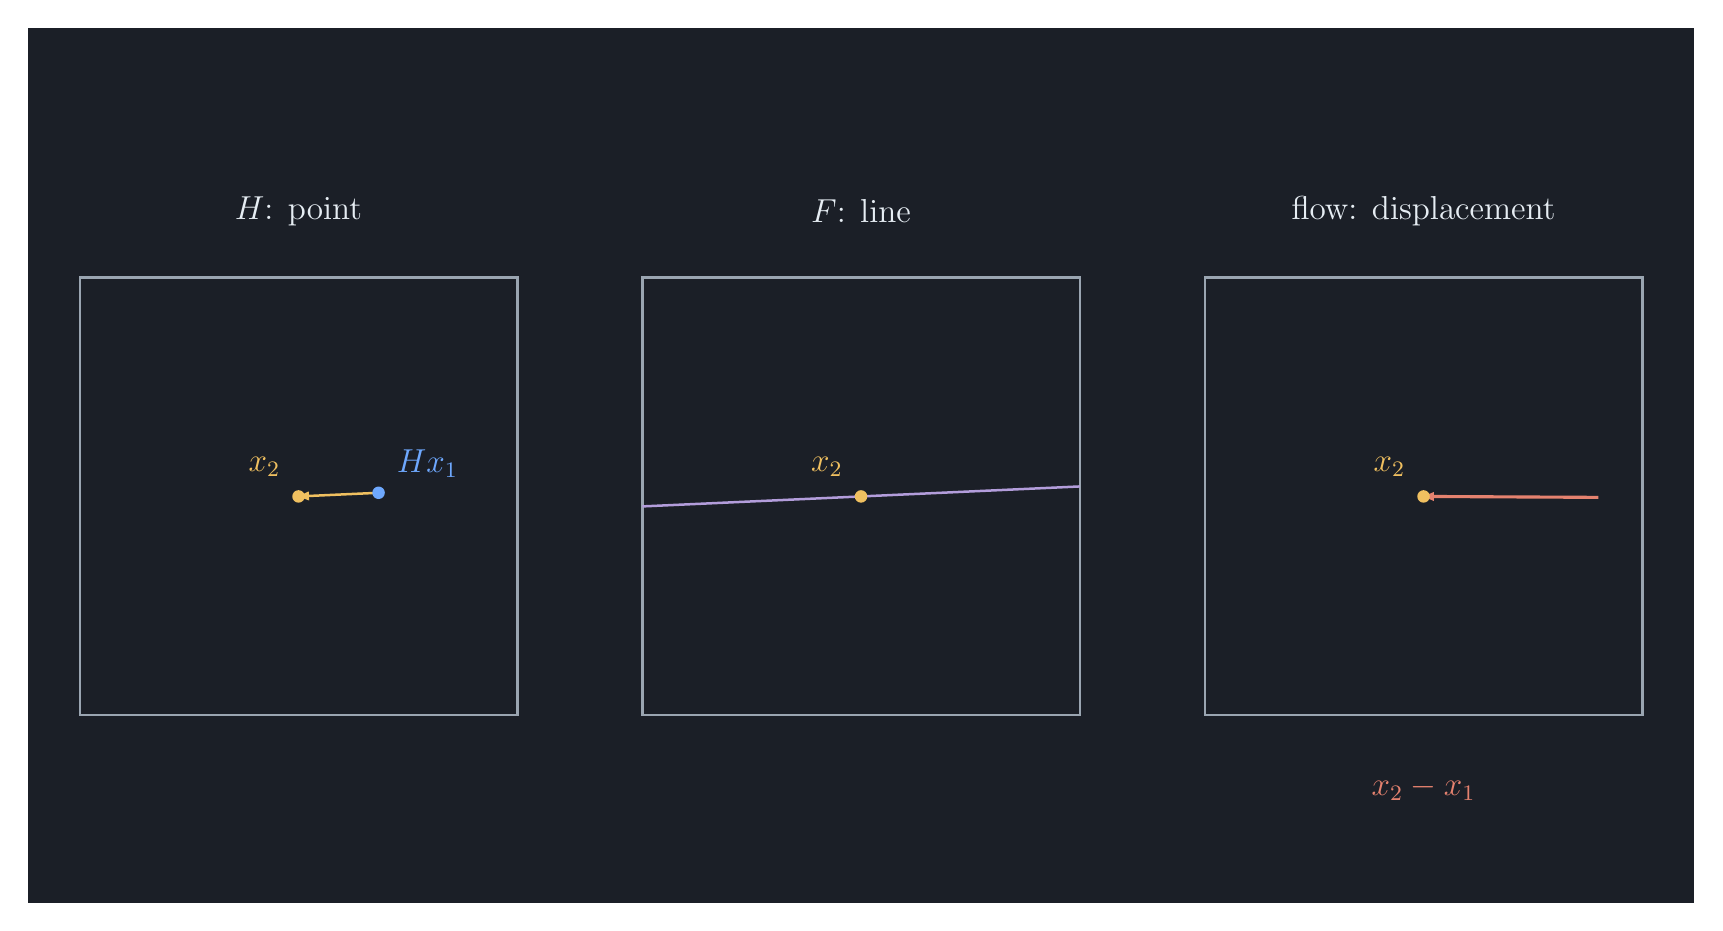
\begin{tikzpicture}[x={(0.026458333cm,0)},y={(0,-0.026458333cm)},every node/.style={font=\fontsize{12}{14}\selectfont}]
\path[use as bounding box] (0,0) rectangle (800,420);
\fill[bg] (0,0) rectangle (800,420);
\path[fill=dim!0!bg,draw=dim,line width=0.9000bp] (25.0000,120.0000) -- (235.0000,120.0000) -- (235.0000,330.0000) -- (25.0000,330.0000) -- cycle;
\path[fill=dim!0!bg,draw=dim,line width=0.9000bp] (295.0000,120.0000) -- (505.0000,120.0000) -- (505.0000,330.0000) -- (295.0000,330.0000) -- cycle;
\path[fill=dim!0!bg,draw=dim,line width=0.9000bp] (565.0000,120.0000) -- (775.0000,120.0000) -- (775.0000,330.0000) -- (565.0000,330.0000) -- cycle;
\draw[observed,line width=0.9000bp] (168.4287,223.2456) -- (130.0000,225.0000);
\path[fill=observed!100!bg,draw=none,line width=0.0000bp] (130.0000,225.0000) -- (134.8945,222.5743) -- (135.0951,226.9697) -- cycle;
\draw[epipolar,line width=0.9000bp] (505.0000,220.2065) -- (295.0000,229.7935);
\draw[c2,line width=1.1250bp] (753.9529,225.4506) -- (670.0000,225.0000);
\path[fill=c2!100!bg,draw=none,line width=0.0000bp] (670.0000,225.0000) -- (675.0117,222.8269) -- (674.9881,227.2268) -- cycle;
\fill[observed] (130.0000,225.0000) circle[radius=2.2500bp];
\fill[prediction] (168.4287,223.2456) circle[radius=2.2500bp];
\fill[observed] (400.0000,225.0000) circle[radius=2.2500bp];
\fill[observed] (670.0000,225.0000) circle[radius=2.2500bp];
\node[text=fg,anchor=center,fill=bg,inner sep=0.4bp] at (130.0000,88.0000) {$H$: point};
\node[text=observed,anchor=east,fill=bg,inner sep=0.4bp] at (122.0000,211.0000) {$x_2$};
\node[text=prediction,anchor=west,fill=bg,inner sep=0.4bp] at (176.4287,209.2456) {$Hx_1$};
\node[text=fg,anchor=center,fill=bg,inner sep=0.4bp] at (400.0000,88.0000) {$F$: line};
\node[text=observed,anchor=east,fill=bg,inner sep=0.4bp] at (392.0000,211.0000) {$x_2$};
\node[text=fg,anchor=center,fill=bg,inner sep=0.4bp] at (670.0000,88.0000) {flow: displacement};
\node[text=observed,anchor=east,fill=bg,inner sep=0.4bp] at (662.0000,211.0000) {$x_2$};
\node[text=c2,anchor=center,fill=bg,inner sep=0.4bp] at (670.0000,365.0000) {$x_2-x_1$};
\end{tikzpicture}
\end{document}
